\documentclass[../resumosTCOM.tex]{subfiles}

\newenvironment{conditions}
  {\par\vspace{\abovedisplayskip}\noindent\begin{tabular}{>{$}l<{$} @{${}={}$} l}}
  {\end{tabular}\par\vspace{\belowdisplayskip}}

\begin{document} 

Linguagens regulares são aquelas que podem ser representadas por DFAs, NFAs, $\epsilon$-NFAs ou REs.

\paragraph{}

\textbf{Pumping Lemma:}
\begin{itemize}
    \item Dada uma linguagem regular infinita L, existe pelo menos um n (pumping length), para cada string \(w \in L\) com comprimento \(|w| \geq n\), podemos escrever \(w = xyz\) com \(|xy| \leq n\) e \(|y| \geq 1 (y \neq \epsilon)\), tal que: \(xy^kz \in L, k = 0, 1, 2, ...\)
    \item Ou seja, podemos encontrar uma string y, que pode ser repetida ou removida, produzindo strings que pertencem à linguagem.
    \item Linguagens finitas são linguagens regulares.
    \item O Pumping Lemma pode ser usado para mostrar que uma linguagem infinita não é regular. Mas não pode ser usado para mostrar que a linguagem é regular.
    \item O Pumping Lemma é uma condição necessária, mas não suficiente para mostrar que uma linguagem é regular.
\end{itemize}

\paragraph{}

Como provar que uma linguagem A é não regular?
\begin{itemize}
    \item Por contradição:
    \begin{itemize}
        \item Assume-se que A é regular.
        \item Como A é regular, tem um pumping length (p).
        \item Todas as strings maiores que p podem ser bombeadas.
        \item Encontra-se uma string s de A tal que \(|s| \geq p\).
        \item Divide-se s em xyz.
        \item Mostra-se que \(xy^iz \in A\) para algum i.
        \item Depois, consideram-se todas as formas de s ser dividida em xyz.
        \item Prova-se que nenhuma das divisões satisfaz as três condições da bombagem ao mesmo tempo.
        \item Logo, s não pode ser bombeada: \textbf{Contradição}.
    \end{itemize}
    \item Condições da Bombagem:
    \begin{itemize}
        \item 1: \(xy^iz \in A\), para todo o \(i \geq 0 \)
        \item 2: \(|y| > 0\)
        \item 3: \(|xy| \leq p\) (pumping length)
    \end{itemize}
\end{itemize}

\paragraph{}

Operações com Linguagens Regulares:
\begin{itemize}
    \item União, Interseção, Complemento, Diferença.
    \item Reverso (\(L^R\)).
    \item Closure (*) e Concatenação.
    \item Homomorfismo e Homomorfismo Inverso (\(L(h(r)) = h(L(r))\)).
\end{itemize}

\paragraph{}

Equivalência de estados e minimização (exemplo):
\begin{figure}[H]
    \centering
    \subfloat{{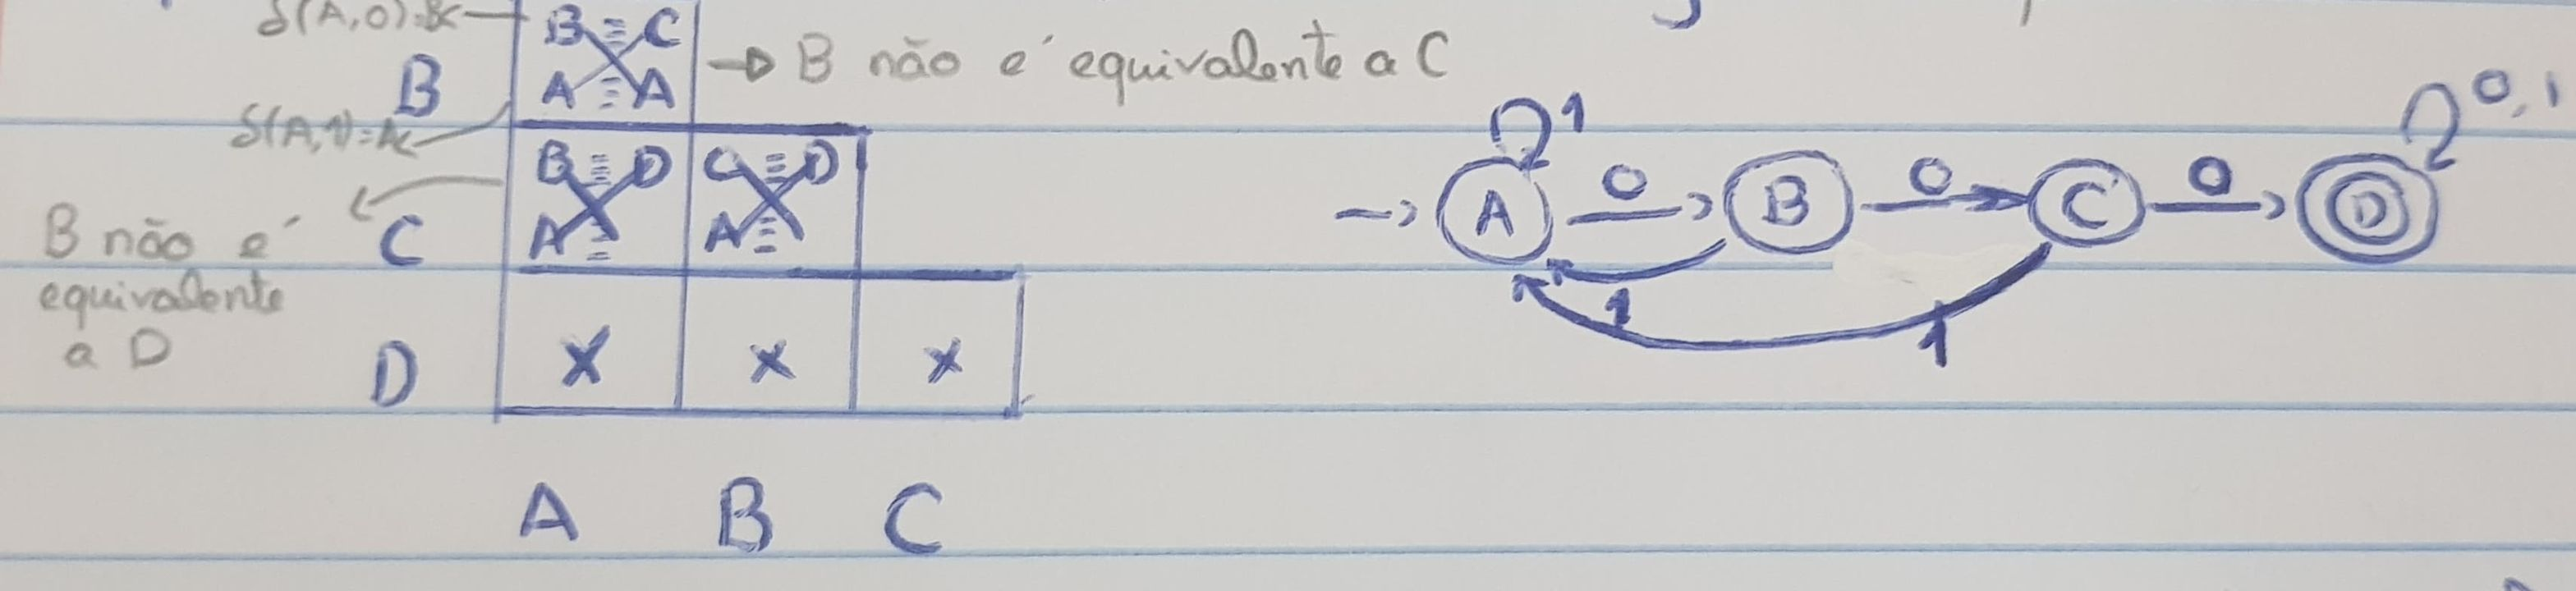
\includegraphics[width=15cm]{images/min_states.jpg} }}%
    \label{fig:nfa_state_min}%
\end{figure}
\begin{itemize}
    \item D não pode ser equivalente a outro estado não final.
\end{itemize}

\end{document}

